% Copyright (c) 2014,2016 Casper Ti. Vector
% Public domain.

\chapter{研究動機}
%\pkuthssffaq % 中文测试文字。
	\section{密碼貨幣的發展}
	追溯著加密貨幣市場的演進,於2009年時,比特幣並非第一個密碼貨幣,在比特幣之前已經有著很多的類似的密碼貨幣開發實驗,但是一直無法做出一個穩定點對點式的電子現金系統,至於製作貧頸會在後段章節中闡述。在比特幣穩定發展之後,有著許多對比特幣有興趣的研究者,以穩定的比特幣系統為基礎修改了許多基本的協議。於2011年相繼創造出了貨幣就稱之為山寨幣,山寨幣早期較為著名的有萊特幣(LiteCoin,LTC)\parencite{litecoin}、狗幣(DogeCoin,DOGE)\parencite{dogecoin}、域名幣(NameCoin,NMC)\parencite{namecoin},於2014年也有人認為比特幣挖礦使用到了大量的哈希運算,這樣的大量運算也浪費了許多的社費資源,努力的開發具有意義的工作量證明挖礦算法較為著名的有素數幣(Primecoin,XPM)\parencite{primecoin}。 於2015年底也誕生了現在最為著名的以太坊經典(Ethereum Classic,ETC)\parencite{ethereumclassic}、以太坊(Ethereum,ETH)\parencite{ethereum},使得區塊鏈技術不再僅僅只是一個點對點的電子現金系統,以太坊最重大突破設計在於將編程語言虛擬機,移植到了區塊鏈架構上,也創造出了屬於乙太坊的編程語言Solidity,使得再以太坊的虛擬機當中,可以用Solidity創建智能合約,合約可以建構去中心化的應用程序,如去中心化的交易所。

	\section{密碼貨幣市場(Cryptocurrency Market)}
	密碼貨幣最具代表性的是比特幣,但除了比特幣之外也有著許多模仿比特幣的密碼貨幣,有的是為了利益,有的是鑒於比特幣的各種不完美,希望可以解決比特幣不足之處。密碼貨幣市場中有成千上萬種的密碼貨幣,較為著名的密碼貨幣會在Cryptocurrency Market Capitalizations\parencite{CryptocurrencyMarketCapitalizations}的排行榜中出現,截至2018年2月8日該排行榜已經收入了1510種密碼貨幣。在Cryptocurrency Market Capitalizations統計的數據當中,可知整體的密碼貨幣市場,如下圖\ref{TotalMarketCapitalization}所示,於2018年1月7日創下了歷史新高,密碼貨幣市場的總市值也高達了829,579,000,000美金,相當於五兆人民幣的總市值。

		\begin{figure}[h]
			\centering
			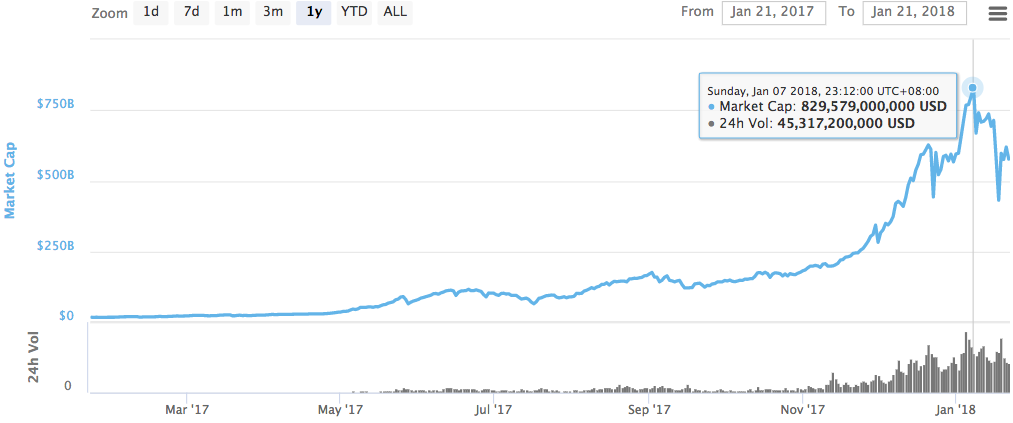
\includegraphics[width = .9\textwidth]{TotalMarketCapitalization.png}
			\caption{Total Market Capitalization\parencite{CryptocurrencyMarketCapitalizations}}\label{TotalMarketCapitalization}
		\end{figure}

	經由Cryptocurrency Market Capitalizations數據顯示,自2013年起已經高達150億美金,2014年與2015年間總市值減少到近乎2013年的一半,於"Have the security flaws surrounding BITCOIN effected the currency's value?."
	論文\parencite{HavethesecurityflawssurroundingBITCOINeffectedthecurrencysvalue?}
	中做了詳盡的比特幣市場調研,致力於探討在各個比特幣市場大事件中對比特幣價格的波動影響,針對影響的程度該論文給出影響指數,當中影響最為嚴重的是於2014年2月發生的日本交易所Mt.Gox倒閉事件,因為早期的密碼貨幣市場中無完善的法律規範,各國對密碼貨幣的接受度有所不同,日本對金融科技的接受度相較較為開放的情況下成立了全世界第一家比特幣交易所,也因為交易所不夠普及,使得大部分的密碼貨幣交易都集中在Mt.Gox交易所中,促使Mt.Gox倒閉事件會成為影響市場價格重大因子之一,也造成2014與2015年的密碼貨幣市場的低迷,2017為2016年的35倍成長幅度,主要是因為美國最大的期權交易中心芝加哥期權交易所於	2017年12月10日支持比特幣期貨,將比特幣價格推升到20,000美金的歷史新高,下圖\ref{Thetotalmarketcapitalization}為2013年至2018年歷年的密碼貨幣總市值的統計圖表。

		\begin{figure}[h]
			\centering
			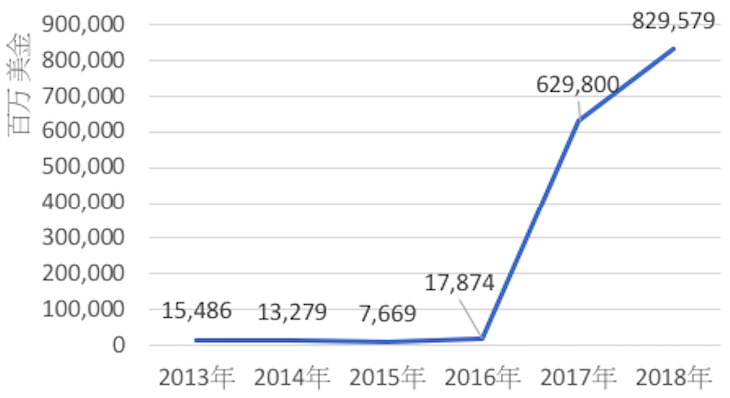
\includegraphics[width = .7\textwidth]{Thetotalmarketcapitalization.png}
			\caption{密码货币历年最高总市值\parencite{CryptocurrencyMarketCapitalizations}}\label{Thetotalmarketcapitalization}
		\end{figure}
	

	\section{密碼貨幣的優勢}
	於2009年Satoshi Nakamoto發布了比特幣系統,成為全世界第一個密碼貨幣的雛形。密碼貨幣的特點在於24小時不間斷運作、遠距離支付、貨幣為使用者持有,區塊鏈技術突破現存傳統中心化金融機構的貧頸。

		\subsection{24小時不間斷運作}
		基於區塊鏈技術與點對點網路的架構,以比特幣為例,自2009年至今,所有的比特幣交易事件皆會儲存在比特幣區塊鏈當中,區塊鏈既無法刪除也無法修改,比特幣區塊鏈會以點對點網路的方式儲存在比特幣網路中的全節點,目前比特幣網路中的全節點高達10552個。與傳統中心化的銀行數據庫相比,可能會因為銀行的服務器維護,導致交易無法順利進行,甚至可能有黑客的入侵導致銀行或是個人資產有重大的損失。點對點網路提供穩定的數據庫資料元,不會因為數據庫的關機而無法繼續使用,
		
		\subsection{遠距離支付}
		於跨國匯款從美國轉帳至中國一百萬美金的場景中,需要經過的手續較為繁瑣,資金有可能需要經過多個國家才可以抵達目的地,在經過各個國家的過程中,需要支付各國的手續費,也需要等待各個國家辦理該業務的時間,既使當資金順利抵達了目的地的銀行,目的地的銀行也需要花將近三至五日的工作日確認該筆金額的來源。屆時領款人亦需要前往銀行完整的身份驗證、解釋資金用途,才得以取得這筆的跨國資金。比特幣系統當中,有著24小時不間斷運作的優點,也因為點對點網路架構,使得比特幣無需經由傳統的金融機構繁瑣的步驟完成國際匯款,於比特幣系統中無系統壅塞的清況下,平均10分鐘即可入帳。

		\subsection{貨幣為使用者持有}
		傳統的金融體系中,資金的存儲、流動往往需要經過銀行,百姓將所有的資產存入銀行,拿到的是一串數字的銀行餘額,銀行是一個中心化的機構,有著最高的權利。中央社的新聞\parencite{Bankguardsstolen}指出,台灣各地於2017年接連於土地銀行、日盛銀行、彰化銀行、京城銀行、兆豐銀行皆傳出銀行行員監守自盜的行為,總金額高達一億三千為新台幣。在比特幣系統中,比特幣有如金幣般存放在個人的比特幣地址當中,使用者為真實持有著貨幣,既使是比特幣系統皆無法動用該筆比特幣資產,唯有比特幣地址的私鑰持有者,才可以移動該筆資產。

		\subsection{開放和透明的交易信息}
			\paragraph{可信任}在公有鏈的基本架構上,所有的交易記錄都是公開透明的,因此交易區塊數據存儲所涉及的所有節點都可以查看交易數據,所有人都可以檢查每個交易記錄的正確性,公開的交易信息使交易數據可信。
			\paragraph{元數據}除了以區塊鏈技術為基礎建構出可信任的系統之外,開放和透明的特性讓更多的開發商或新公司更容易獲得交易的原數據。畢竟,在傳統金融體系中,所有交易記錄均由中央金融機構存儲。從中央金融機構提取原始交易信息並不容易,區塊鏈的開放性和透明性促使金融公司降低了獲取原始數據努力的門檻。公司或學者可以製定一個可視化的開發計劃,甚至可以使用大量數據來分析以前從未見過的有價值的觀點。

		\subsection{區塊鏈交易數據無法修改和刪除}在區塊鏈結構中,通過嚴格驗證的所有信息都記錄在區塊鏈中無法刪除。 根據區塊鏈的特點,舊區塊的哈希值在連接區塊鏈的過程中存儲在新區塊中,只要塊中的值被修改,即使有一點,也會使哈希值完全不同,也就是說,雪崩效應將會發生。由於這種結構,所有的信息都不會被改變,所以如果驗證的結果被改變,該塊將不被系統接受。因此,所有的交易記錄已經存儲在區塊鏈中,不能修改和刪除。

		\subsection{匿名}在當今社會,個人信息保護已成為企業最重要的問題。在區塊鏈系統中創建的所有賬戶都不會與真實世界中的實體建立直接關係,因次建立匿名。區塊鏈系統中的所有賬戶都是由單獨的匿名個人創建的,可以有效保護消費者的隱私。然而,Visa交易是不同的,我們會向Visa公司的集中主機顯示大量個人信息,這可能會導致個人信息洩露的風險。在區塊鏈技術中,可以經濟有效地避免這個問題。

		\subsection{自治系統}
		在區塊鏈系統中,操作依賴於一些算法,包括一致性算法。因此,在這種自治系統中,沒有人(例如節點或礦工)可以直接改變係統操作的規則。如果在比特幣系統中發現需要更正的嚴重錯誤,可以建議使用比特幣改善提案(Bitcoin Improvement Proposals,BIP)升級比特幣系統。 在升級模塊可以在比特幣系統上正式運行之前,提議的比特幣改進建議需要得到比特幣系統中超過一定數量的礦工的支持。由於這種以投票機制升級系統的門檻相當高,使得區塊鏈系統通常不會有大的變化,但相對穩定。

	\section{密碼貨幣的劣勢}
	在區塊鏈技術中,有著幾項貧頸,每秒處理的交易量(Transactions Per Second,TPS)上限、無法達成即時交易確認、洗錢防制困難、低可擴展性。

		\subsection{每秒處理的交易量(Transactions Per Second,TPS)上限}
		下圖\ref{TPS}為VISA為國際上最為著名的支付系統,以中心化運營的方式,可以支持高達2,000筆交易每秒。但是以區塊鏈技術為基礎的比特幣最大能夠接受的每秒處理的交易量僅為7筆,這樣的上限由許多原因造成。

			\begin{figure}[h]
				\centering
				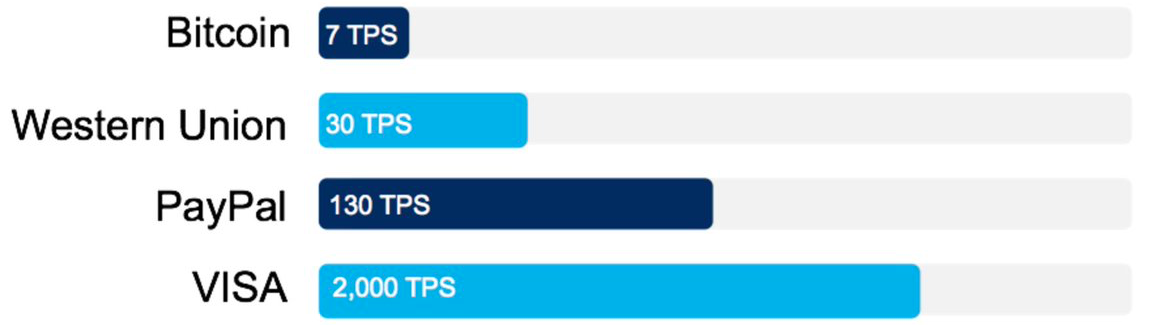
\includegraphics[width = .7\textwidth]{TPS.png}
				\caption{每秒處理的交易量 比較圖\parencite{TPS}}\label{TPS}
			\end{figure}

			\paragraph{上修區塊大小上限,區塊鏈成長速度過快會造成去比特幣全節點不堪負荷}
			從2009年至今的比特幣區塊鏈大小已達到156GB,這樣的成長速度因為比特幣區塊大小的最大值被設置為1MB。下圖\ref{blockchainsize}為過去比特區塊鏈大小,圖中可以發現,於2016年開始,比特幣區塊鏈的成長速度為一直線,這表示著比特幣網路中持續的維持在公不應求的狀況。現今對比特幣的每秒處理的交易量有許多優化的方案,包括解除比特幣區塊大小1MB的限制。在一個區塊上限為1MB的限制下,滿載的比特幣系統中,比特幣區塊鏈平均每十分鐘會增1MB,每小時會增加6MB,每天會增加144MB,每月會增加4.2GB,每年會增加高達50GB,要達到1TB的區塊鏈大小還需要8年,在8年後的未來存儲1TB的數據量應該不會有太大的負擔。倘若解除1MB的區塊限制,在系統的每秒處理的交易量看似可以接受更多的交易成倍成長,面臨1TB的比特幣區塊鏈數據會在更短的時間內出現,倘若存儲區塊鏈特成本超過了摩爾定律的成長曲線,會進一步造成自願成為比特幣全節點的意願度降低,使得比特幣網路的全結點數變少,促使比特幣去點對點網路往中心化網路發展,失去一開始點對點網路的意義。

			\begin{figure}[h]
				\centering
				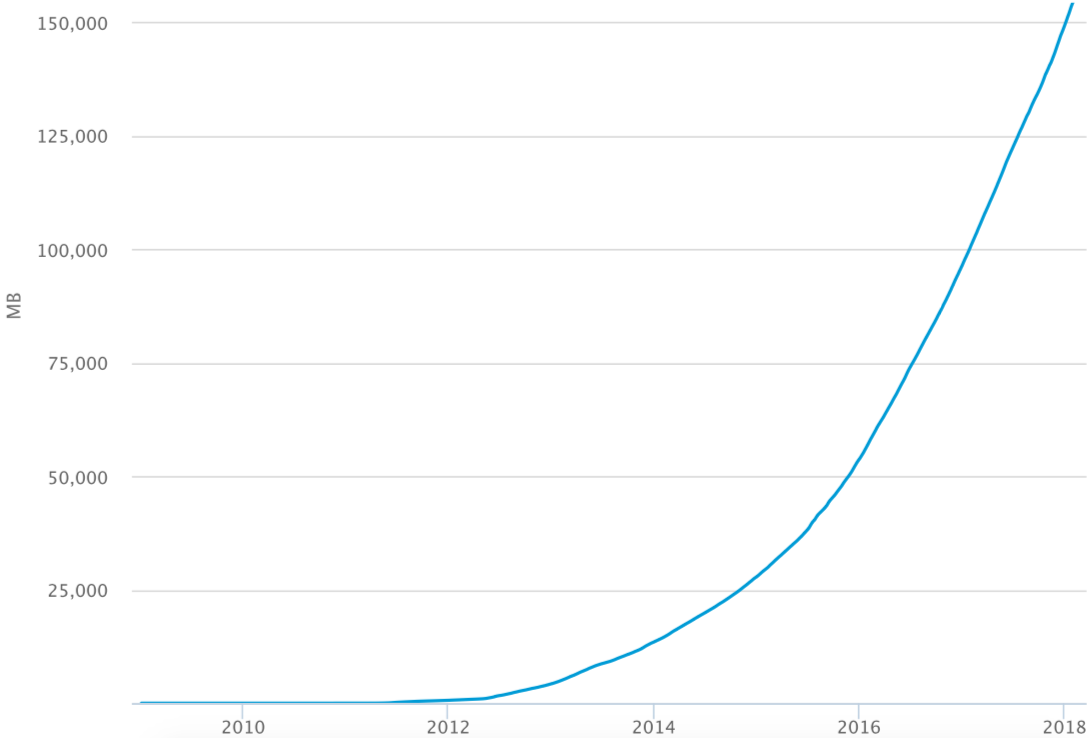
\includegraphics[width = .7\textwidth]{blockchainsize.png}
				\caption{比特幣區塊鏈大小\parencite{blockchainsize}}\label{blockchainsize}
			\end{figure}

			\paragraph{上修區塊大小上限,造成區塊鏈最新區塊同步延遲}
			對於區塊鏈的區塊同步延遲造成比特幣網路的影響,於“Increased block size and Bitcoin blockchain dynamics”\parencite{TelecommunicationNetworksandApplicationsConferenceITNAC201727thInternational}有著詳細的研究,在上修區塊大小上限的議題上,除了造成比特幣全節點意願度下降,亦有機會造成以比特幣點對點網路建構出的區塊鏈同步上造成延遲,在1055個比特幣全節點當中,平均每十分鐘會有礦工於其中一個全節點生成一個最新的區塊,該最新的區塊會以點對點網路協議同步到1055個節點上,在比特幣系統中,長年來的實驗可以發現在礦工生成1MB的區塊後同步到全網節點可以在創造下一個區塊前完成。倘若將區塊大小修改為2MB或是更大,會使得比特幣全節點的最新區塊同步延遲的現象更加的明顯,同步延遲會使得區塊鏈分岔,造成1055個比特幣全節點的信息不一致,近一步造成整得比特幣點對點網路崩潰。

		\subsection{洗錢防制困難}
		匿名性為比特幣系統一大特色,比特幣的地址生成是在$2^256$的組態空間中隨機選取,這樣的地址與現實生活中的身份並無任何關聯,使得黑市交易、洗錢防制邊的困難,甚至有更為前沿的密碼貨幣Monero導入了環簽章算法、Zcash導入零知識證明算法\parencite{Zero-KnowledgeProofsofIdentity},使得原本公開透明的區塊鏈,變得無法檢視,使得密碼貨幣在洗錢防制上更加的困難。論文"An Analysis of Bitcoin Laundry Services."\parencite{AnAnalysisofBitcoinLaundryServices},致力探究比特幣匿名交易下的資金流動模型,試圖以機械學習的方法找出比特幣洗錢模型作為洗錢的工具,下圖\ref{Darklaunderworkflow}為該論文針對黑市交易中的洗錢服務運營商Darklaunder進行洗錢機械學習識別。

			\begin{figure}[h]
				\centering
				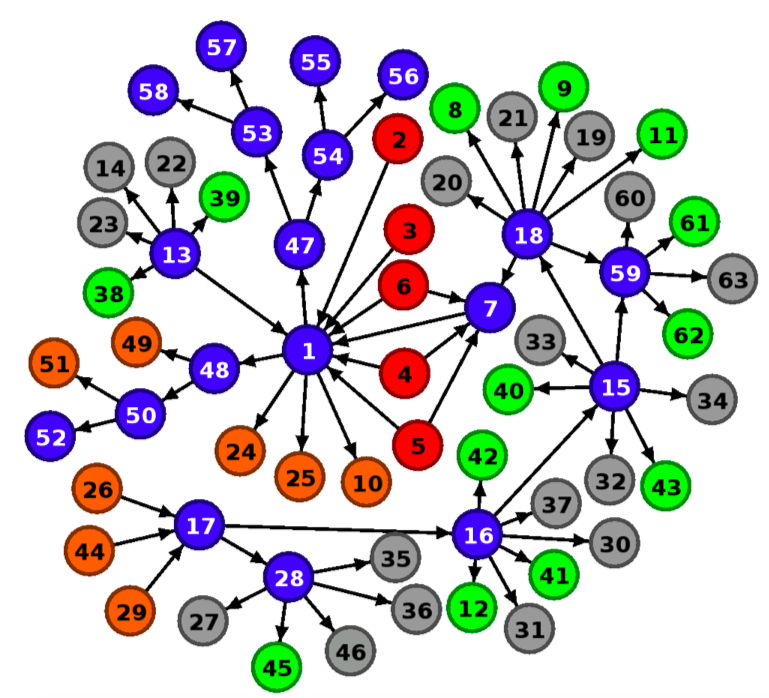
\includegraphics[width = .7\textwidth]{Darklaunderworkflow.png}
				\caption{Darklaunder 洗錢模型\parencite{AnAnalysisofBitcoinLaundryServices}}\label{Darklaunderworkflow}
			\end{figure}

		\subsection{低可擴展性}
		\paragraph{修改比特幣協議製作添加外部信息的區塊鏈}比特幣區塊鏈技術是一個嚴謹的架構,倘若要創造可以支持外部信息的結構需要重新創造全新的貨幣,大部分的密碼貨幣皆不支持外部輸入,外部的信息輸入皆無法保證資料的正確性,近一步造成垃圾勁垃圾出的問題,倘若錯誤的信息存儲在無法刪除、修改的區塊鏈下,只是強化該筆錯誤信息的錯誤。
		\paragraph{於區塊頭或交易信息添加外部信息} 比特幣區塊鏈上,可以添加一些信息於區塊上,開信息會永久保存於區塊鏈上,除了在區塊上新增信息,在比特幣單筆交易信息上,亦可填寫一些私人信息,但這樣的空間大小有限,且現今的比特幣價格日趨上漲,比特幣交易手續費是以單筆交易大小計算,使得在交易中添加些個人信息變得更加昂貴。

		在比特幣系統中,其區塊鏈僅用於記錄交易記錄,不能擴展更多功能和應用程序。有很多開發者希望將比特幣系統擴展到智能合約等其他應用程序。但是,他們後來發現這是基於原始比特幣系統框架的具有挑戰性的工作。因此,全球第二大數字貨幣Ethereum的作者Vitalik也創建了Ethereum虛擬機。 所以,創建的智能合約可以在統一的以太坊平台上運行。 以太坊打破了比特幣的技術瓶頸。

% vim:ts=4:sw=4
